\section{Background}

\subsection{Disaggregated Memory}

Memory disaggregation separates primary storage from the CPU
by a fast network. The question \textit{how to present
memory over the network to an application?} is still open,
and a spectrum of system designs currently exist.
Transparent systems present far memory to the application as
if it were local. Virtual memory enables paging systems to
keep a cache of local pages, and swap in and out
transparently on page faults ~\cite{infiniswap, leap,
fastswap}.  Some have argued that page granularity is too
course and built upon an incoherent caching
layer~\cite{kona, legoos}.  In both cases transparency
incurs a performance cost as remote accesses cannot be
optimized for by the running application.
%%
Alternatively applications can access remote memory
explicitly with an API similar to an RPC
call~\cite{aifm,reigons,clover,sherman,faast}. Explicit
access allows for optimized remote requests. They can be
batched, scheduled, and managed by libraries and runtimes. 
%%
Whether explicit or transparent sharing is expensive, at the
time of writing no transparent system supports shared memory
-- the cost of cache coherence is prohibitively high in
terms of bandwidth and latency. Explicit cases are more
promising for sharing as they allow application developers
to acquire locks, and for libraries to make use of
optimistically concurrent datastrcutrues.

\subsection{RDMA protocol}

RDMA provides an interface for accessing remote memory. It
provides a set of zero copy instructions (\textit{verbs})
which are initiated by a client cpu. NICs manage the entire
network stack including control flow, reliable delivery, and
at most once semantics. The guarantees RDMA provides are
configurable -- connection's UDP like semantics are provided
by Unreliable Datagram (UD) and Unreliable Connections (UC),
while Reliable Connections (RC) at similar to TCP, ensuring
in order delivery, and enabling RDMA's one-sided operations
Read, Write, and Compare and Swap (CAS).

Which connections to use is an intense topic for debate.
Reliable connections use NIC memory, a precious resource,
and projects designed using Mellanox CX3-CX5 noted that RC
bottlenecked scalability due to memory and cache
limitations~\cite{farm,faast,erpc,litem,design-guidelines}.
While host memory can provide better scalability modern NICs
have bigger caches with better cache
management~\cite{storm}. In the disaggregated setting no
memory side CPU exists to manage the state making RC the
only option for one sided operations.

\todo{connection multiplexing ~\cite{flock}}
\todo{RDMA middlebox (find citaitons ~\cite{mind,switchml})}

%% RDMA

% Remote direct memory access (RDMA) is a network protocol
% which allows NICs to bypass CPUs and access host memory
% directly.  The RDMA protocol consists of a set of verbs
% which abstract remote memory instructions. Instruction
% execution and connection state are entirely managed by the
% NIC which exposes the verbs API to the CPU. The CPU
% registers memory regions for DMA with the NIC and sets up
% connections (Queue Pairs) with a remote RDMA enabled NIC.
% %%
% RDMA connections come in a variety of flavors, each of which
% enables a different set of RDMA verbs and delivary
% guarantee~\cite{herd, erpc, storm}. Unreliable Datagram
% (UD), and Unreliable Connection (UC) operate similar to UDP
% with no reliable delivery or ordering guarantees and a
% restricted set of verbs.  Reliable Connected (RC) operates
% similar to TCP, the NIC manages connection states for each
% QP and ensures reliable in-order delivery by using sequence
% numbers and a go-back-n retransmission protocol.
% %%
% Serious debate exists over which connections to
% use~\cite{storm,cell,herd,faast,farm}, each has advantages
% and disadvantages in terms of NIC resource utilization,
% throughput, and latency. Disaggregated architectures have no
% remote CPU's, in this proposed setting RC is the most
% attractive as it alone enables the use of one-sided verbs
% :\textit{Read}, \textit{Write}, and the atomic \textit{CAS}
.


%% RDMA Connections
%% RDMA Atomics

\subsection{Programmable Switches} Most proposals for
disaggregation are at rack-scale. They propose a single rack
with servers partitioned into roles: compute, memory, and
storage, each of which is interconnected by a TOR.  The TOR
is central in this architecture, a fact which has not gone
unnoticed by system designers who argue that a programmable
switch can facilitate remote memory apis, and OS
functionality~\cite{disandapp,mind}. 
%%
Literature on offloading OS, and service level functionality
to programmable switches is
plentiful~\cite{netlock,netkv,netchain,netcache}. The
constraints in each case are similar, switches have limited
memory, and processing capabilities, if the computational
ask of the switch is too high packets must be recirculated
adding additional latency, and reducing aggregate bandwidth.
Ideal applications for programmable switches use little
memory, require little processing and enable a huge
performance benefit from centralization, and the billions of
operations (in terms of packets) that a switch can process
per second.
%%
Prior work has shown that programmable switches are able to
manage locks~\cite{netlock}, track the state required to
maintain an RDMA reliable connection~\cite{tea}, and provide
rack scale serialization at low
cost~\cite{eris,no,when-computer}. These properties make a
top-of-rack programable switch ideal for managing remote
memory as it can guard access, maintain connections, and
provide serialization primitives for all clients.


\section{Serialization}

\begin{figure}[t]
  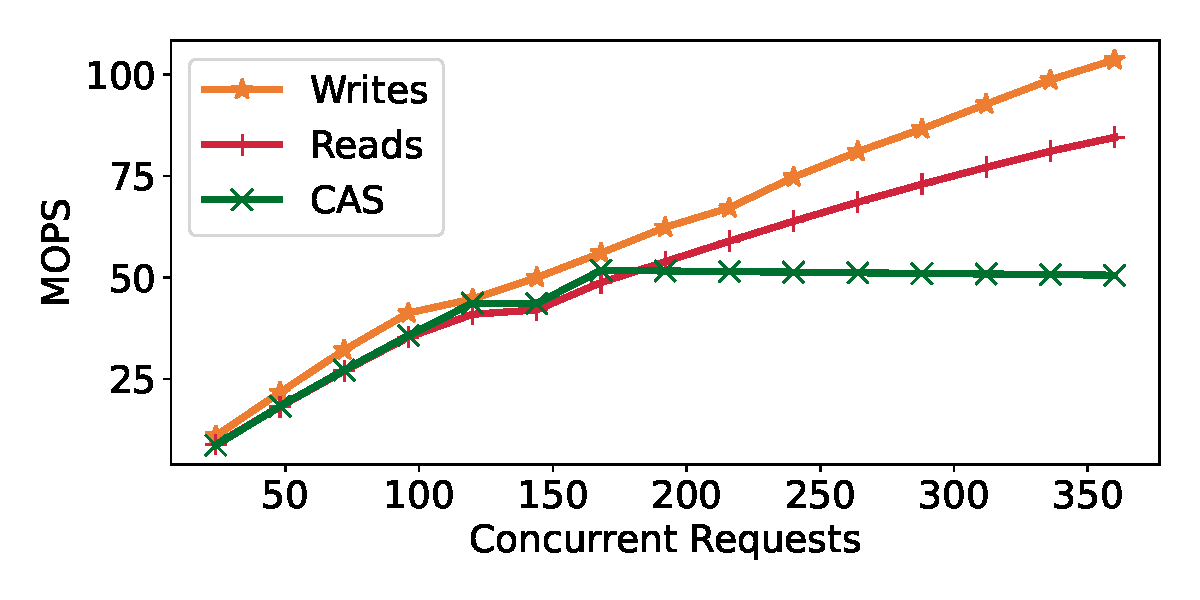
\includegraphics[width=0.485\textwidth]{fig/rdma_concur.pdf}
  \vskip -0.5em

    \caption{Achieved throughput of RDMA verbs across twenty queue
      pairs on data-independent addresses as a function of request
      concurrency.  When using atomic requests, ConnectX-5 NICs can
      support approximately 2.7 MOPS per queue pair, up to about 55
      MOPS in aggregate.}

    \label{fig:rdma_concur}
      \vskip -0.5em
\end{figure}

\begin{figure}[t]
    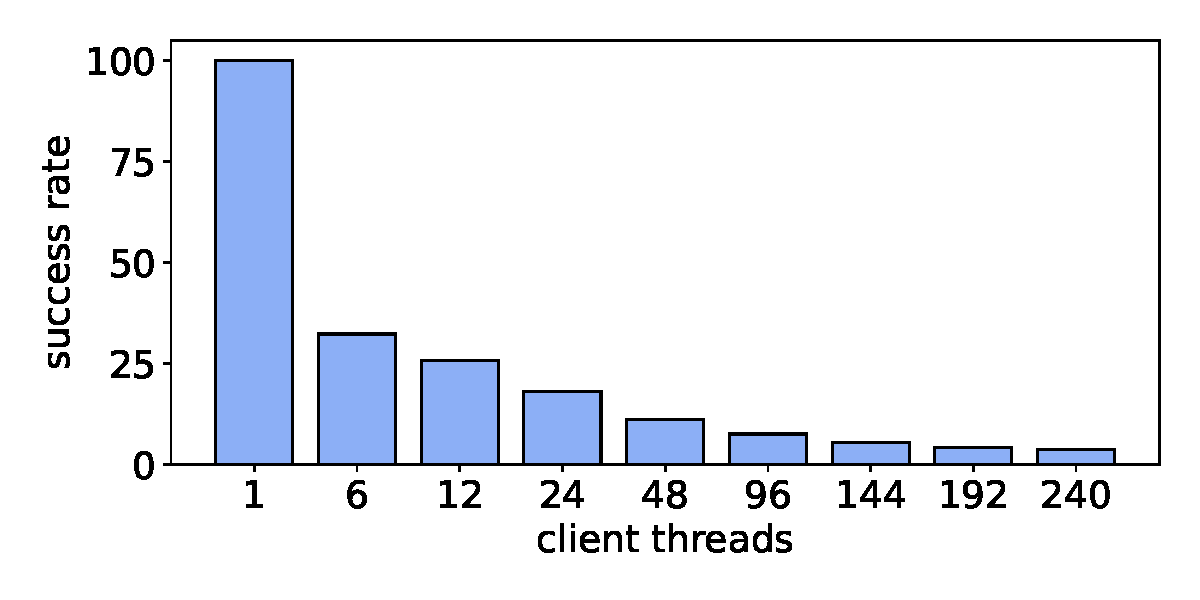
\includegraphics[width=0.485\textwidth]{fig/success_rate.pdf}
    \vskip -0.5em
    \caption{Percentage of successful operations in a
      50:50 read-write workload spread across 1,024 keys according
      to a Zipf(0.99) distribution as more client threads are
      added. At 240 threads less than 4\% of operations succeed.}
      
    \vskip -0.5em
    \label{fig:success_rate}
\end{figure}

\begin{figure}[t]
  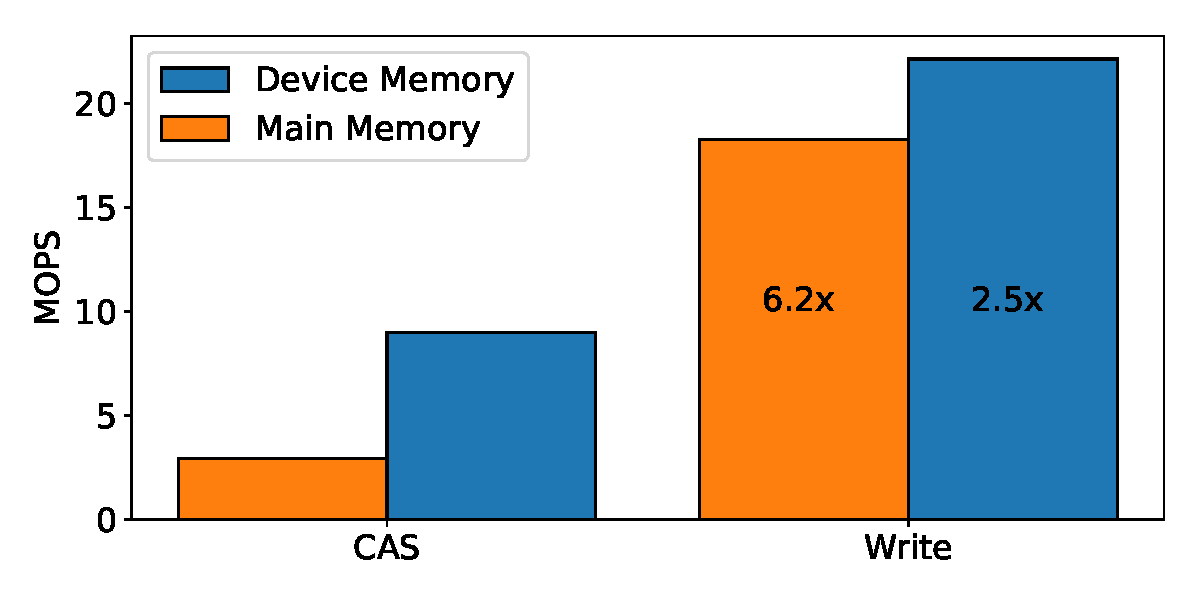
\includegraphics[width=0.485\textwidth]{fig/cas_vs_writes.pdf}
%  \vskip -0.5em

  \caption{ Throughput comparison of serialized RDMA operations in
    NIC-mapped device and main memory. Writes obtain 6.2$\times$ higher
    throughput than CAS in host memory and 2.5$\times$ higher in NIC memory despite being restricted to a single queue pair.  }

    \label{fig:cas_vs_writes}
%      \vskip -0.5em
\end{figure}

\subsection{RDMA serialization} RDMA atomics instructions
serialize remote memory operations without the need for a
memory side CPU. These instructions \textit{Fetch-and-Add}
and \textit{Compare-and-Swap} (CAS) execute on 64 bit width
words and are guaranteed to have atomic visibility across
all queue pairs. These operations are expensive. On a single
address atomic instructions can only execute a few million
operations per second, each operation forces a blocking PCIe
round trip.  As a performance mitigation Mellanox NICs
supply a small (few KB) region of device mapped memory which
allows the memory side NIC to execute RDMA instructions on
it's local device memory without incurring a PCIe round
trip~\cite{sherman}. Executing atomics on this memory is 3x higher
throughput than host memory, but still slower than it's read
and write counterparts~\ref{fig:cas_vs_writes}.  Across
independent addresses they have approximately half the
throughput of their non atomic
counterparts~\ref{fig:rdma_concur}. 
%%
Data structures built with RDMA atomics have hard
performance limits because the aforementioned constraints.
Locks located at a single address which use traditional
lock, unlock operations are limited to around 500k accesses
per second. This assumes perfectly coordinated requests,
under contention requests which fail to acquire or release a
lock still consume operation bandwidth.
%%
Under contention RDMA has poor support for traditional
locking. In contrast optimistic data structures with locks
scattered throughout, such as a linked list, are not rate
limited by this single address restriction.  However, they
are fundamentally limited by the fact that any atomics have
half the throughput of reads and writes. More critically,
under contention optimistic data structures have no liveness
guarantees under contention atomic operations fail
frequently (Figure~\ref{fig:success_rate}).  RDMA has no
support for resolving pointers (pointer chasing) and
retrying operations for such data structures(~\cite{rma}), a
simple operation usually executed by a memory side CPU. As
such RDMA clients are forced to resolve their failures
requests themselves often retrying many times.
%%
Atomic operations are not the only serialization mechanism
provided by RDMA. Reliable connections provide in order
delivery on individual queue pairs. This allows clients to
issue multiple requests in parallel and allows the NIC to
resolve reordering and dropped packets using go-back-n This
allows clients to issue multiple requests in parallel and
allows the NIC to resolve reordering and dropped packets
using go-back-n retransmission. When clients are collocated,
queue pairs can be shared by multiple cores through
techniques like flat combining~\cite{flock,sherman}. This
technique removes the need for RDMA atomics, as clients can
locally resolve their conflicts and then issue their
requests to remote memory at the full throughput of reads
and writes. Unfortunately this technique is not applicable
to distributed clients as they do not share access to the
same queue pair

\subsection{Programmable Switch Serialization}

Switches can cheaply serialize packets~\cite{when-computer}.
Programable switches with P4 pipelines can use this cheap
serialization, along with their ability to manage small
amounts of state in network, to serialize distributed
applications. Mind for instance provides a unified TLB and
cache for disaggregated applications~\cite{mind}. Packets
processed by a programmable switch are sequenced in order,
updates to the switches registers are atomic with respect to
the packets as each state of the pipeline is occupied by
exactly one packet at a time. A centralized switch can
therefore apply monotonic sequence numbers to a stream of
packets, or maintain a lock without the need for explicit
atomic operations.

Unfortunately this serialization is not sufficient for RDMA
memory operations out of the box. RDMA packets on two
reliable connections may be ordered on the switch, and then
subsequently reordered by the receiving side NIC, or by the
PCIe bus~\cite{understanding-pcie}.

In all cases switch memory and compute are highly
constrained. Any operations that exceed the processing
limit of the match action pipeline require recirculation
which consumes additional switch bandwidth. For example,
terminating connections with a switch is prohibitively
expensive as both the state of the entire connections, and
the logic for connection startup and teardown would consume
large quantities of the switches buffers. Any logic, or data
offloaded to a programable switch must therefore be minimal
in order to meet the compute and data restrictions of the
switches SRAM.

\section{Swordbox}

We present \sword a middlebox solution for sharing remote
memory. \sword provides acceleration for both lock based and
optimistically concurrent data structures. Locks are managed
in network, and the results of locking operations are
forward to memory. Lock accesses are accelerated by
replacing RDMA atomic operations with writes in flight.
Modified lock operations are multiplexed onto existing RDMA
connections, per lock, to ensure serialized access to the
lock. \sword also provides a mechanism to remove contention
from optimistic data structures by caching the metadata
required to detect and resolve conflicts. These techniques
are implemented in a DPDK prototype for the lock based
approach and fully realized in P4 for optimistic data
structures. Figure~\ref{fig:system} shows the overall design
of swordbox.

\subsection{Locks}

\sword caches locks and forwards the result of locking
operations to remote memory. Storing locks in switch memory
enables 10's of millions of lock and unlock operations per
second~\cite{netlock}. At these rates CAS on single
addresses is the bottleneck. \sword serializes lock
access and forwards the results to the servers, therefore
the application CAS operation can be modified to a simple
write as the result is known prior to arriving at the memory
side NIC. On an individual QP this modification is safe --
across QP however reordering can occur between the switch
and memory. We therefore multiplex lock operations onto
shared QPs.
%%
Swordbox manages reliable connections for all connected
clients. When clients first connect \sword detect the
connection startup and tracks the sequence numbers on that
connection. The total number of active connections is
tracked as well. When a lock acquire or release issued \sword
take the lock address \textit{mod} it's address and assigns
it to a connection. This ensures that all operations to the
same lock are placed on the same reliable connection.
%%
When a CAS for a known lock passes through \sword it checks
it's lock table and calculates the result of the locking
operation, (aquired, released or failed). The RDMA packet
then has it's operation value changed from CAS to Write, and
is assigned to the downstream reliable connection the lock
was mapped to. Each request must be multiplexed and
demultiplexed, when a lock request is assigned to a stream
it has it's QP, and sequence number updated so that the
receving side NIC is unaware that any modification have been
made in network. A stub of the mapping is stored with
relation to the connection, when a response from the NIC
returns from the switch the packet has it's sequence number
mapped back to it's original value, and is mapped back to
it's original sender. For each mapped request the switch
must store both a sequence number and the id of the
requesting client. 
%%
Our systems support only closed loop clients which issue one
request at a time, and are guaranteed to retry requests lost
in transit. Using this assumption the amount of state the
switch needs to store is bounded by the number of clients.
It must store a sequence number for each client QP, and
stubs for each outstanding request. This requires at most 2
24 bit sequence number for each client.

\sword assumes that locks are located at well known
location. Logic for managing locks is application specific
and implemented in \sword. No modification to the client is
required as \sword operates directly on RDMA packets, using
their QP id's and virtual addresses. In Sherman for instance
locks are mapped to a special region of NIC memory with a
well known virtual address range.

\subsection{Optimistic Concurrency}

Lock based data structures are limited under contention both
by the rate at which locks can be acquired, and by the size
of the critical section each client must execute. Under
severe contention the critical section is the bottleneck.
Optimistic strategies differ in that work completed in
scratch memory, and then committed via an atomic operation
like CAS. 

Take for example a linked list which supports an append
operation. Clients running append must first write the
value of the node they wish to append, and then commit to
the list by running a CAS which modifies the null pointer at
the end of the list to then point to the new entry. Such
strategies require no lock acquisition but still struggle
under contetion. If the end of the list is continuously
being appended to and multiple clients are in a race, one
will succeed, the others will fail, need to traverse the
list to the new tail, and reissue a request. This is the
exact scheume Clover uses to handle writes to its persistant
key value store. Clover operates well under read only
workloads but struggles under contention as the tail of each
list moves faster clients must repeatadly chase thye tail
pointer of the list, each read requiring a round trip.

\sword is designed to entirely remove contention in
optimistic concurrency schemes like those found in Clover.
As all requests are serialzed \sword can observer the most
up to date location of the lists tail. We cache this value
and use it to resolve conflicts. When requests arrive at
sword which append to the tail of the list, the virtual
address of the tail is stored for that key. This requires
storing one 64 bit virtual address for each key in the key
value store. While this overhead may seem large, \sword need
only store hot keys. Uncontended keys can simply be written
and read using clovers default protocol. When requests for a
key arrive at \sword it looks up the value of the write and
determines the location of the lists tail. If the request is
pointing to the tail, the in network cache is updated and
the request is forwared to memory with no modification. If
the request is out of date (directed to an interior node of
the list) \sword modifies the virtual address of the CAS and
forwards it to the known tail location, updating it's own
cache in the process.

This strategy remotes all contention from Clover and
requires not modifications to the application itself. A key
aspect of this approach is that Clover has end to end
recovery and does not rely on \sword to complete requests.
If a key is not tracked by \sword then the request is
forwarded directly to memory with no modifications. Our
prototype statically tracks hot keys, however a dynamic
solution in which hot keys are detected via a count min
sketch are well within the capabilities of future
versions~\cite{switchml}.